\noindent
\section{Dataset}
\label{dataset}
We consider datasets of two physics journals (i) Journal of High Energy Physics (JHEP) and 
(ii) Journal of Statistical Mechanics: Theory and Experiment (JSTAT). JHEP is a leading physics 
journal with an impact factor of 6.023\footnote{http://iopscience.iop.org/journal/1126-6708} and 
publishes theoretical and experimental papers in high energy physics while JSTAT publishes papers in statistical physics and has 
an impact factor of 2.091\footnote{http://iopscience.iop.org/journal/1742-5468}. 
JSTAT is more interdisciplinary and attracts papers from a wide range of researchers from physicists to computer scientists while for JHEP the papers published are 
limited to only very specific topics. 
Note that these are two diverse datasets; while JHEP predominantly follows a single-referee format with only around 10\% papers being reviewed by multiple referees, 
JSTAT is more open to a multiple-referee format (close to 43\% papers are multi-refereed). 

\noindent{\bf JHEP} dataset contains information of 28871 papers which were submitted between 1997 and 2015. The meta information available for each paper includes 
(i) the title, (ii) the list of authors, (iii) the final decision (accept/reject/withdrawn), (iv) the keywords related to the paper, (v) the long term citation 
(cumulative citations received 
from date of publication to 2015), (v) the submission date, (vi) the publication date (in case the paper was accepted) and (vii) the abstract. 
Moreover, for each paper the whole review process information is available which includes (i) the assigned editor, (ii) the assigned reviewers, (iii) the report submitted 
by the reviewers in each round of review and (iv) the citation information of the accepted papers.
%We also obtain the citation information of the rejected papers by querying the inspire database\footnote{http://inspirehep.net/?ln=en}. 
%Some general information related to the JHEP dataset is noted in 
%table \ref{tab:data}.

\noindent{\bf JSTAT} dataset contains information of 6106 papers which were submitted between 2004 and 2016. The meta information available for each paper is same as that of the 
JHEP dataset. 
All the above information for both the datasets were made available to us by the respective publishing houses.

\noindent{\bf Information crawled:} For JHEP we further queried the $inspire$ database\footnote{http://inspirehep.net/?ln=en} to obtain citation and other meta information 
of the rejected papers.  
For JSTAT the citation information of the papers (both accepted and rejected) were not available. Hence, we collected the titles of all the papers and queried the ``scopus''\footnote{https://www.scopus.com/home.uri}
database to obtain the citation information of the papers (both accepted and rejected). 
Note that this is the long term citation i.e., the cumulative citations received from the date of publication to 2016. Throughout the paper any reference to citation 
would mean this cumulative citation unless otherwise specified.
%Since we have the titles for both the accepted and the rejected papers, we could crawl the citation information for both these classes. 
Some general information related to the two datasets is noted in table~\ref{tab:data}.
Further, for both JHEP and JSTAT, each paper is assigned a set of keywords (at least 2 and at most 4) by the publisher which represents the related topic of a paper. 

%\textcolor{blue}{Sandipan: It was there for JHEP but not for JSTAT. Rejected papers were tracked through the tile and author list.}
%table \ref{tab:data}.
% \begin{table}[]
% \centering
% \caption{Some general information related to the two datasets.}
% \label{tab:data}
% \begin{tabular}{l|l|l}
% \hline
%                                                                                       & JHEP  & JSTAT \\ \hline\hline
% \# papers                                                                             & 28871 & 6106  \\ \hline
% \# accepted papers                                                                    & 20384 & 3528  \\ \hline
% \begin{tabular}[c]{@{}l@{}}Fraction of multi-reviewed \\ papers\end{tabular}           & 0.12  & 0.43  \\ \hline
% \begin{tabular}[c]{@{}l@{}}\# Editors with at least one \\ assignment\end{tabular}    & 95    & 148   \\ \hline
% \begin{tabular}[c]{@{}l@{}}\# Reviewers with at least \\ one assignment\end{tabular}  & 3976  & 2647     \\ \hline
% \begin{tabular}[c]{@{}l@{}}Average number of \\ reviewers per paper\end{tabular}      &  1.03     & 1.42      \\ \hline
% \begin{tabular}[c]{@{}l@{}}Average number of \\ authors per paper\end{tabular}        &  2.87     & 2.32      \\ \hline
% \begin{tabular}[c]{@{}l@{}}Average number of \\ assignments per reviewer\end{tabular} &  6.48     &  2.56     \\ \hline
% \end{tabular}
% \end{table}

\begin{figure}
 \centering
 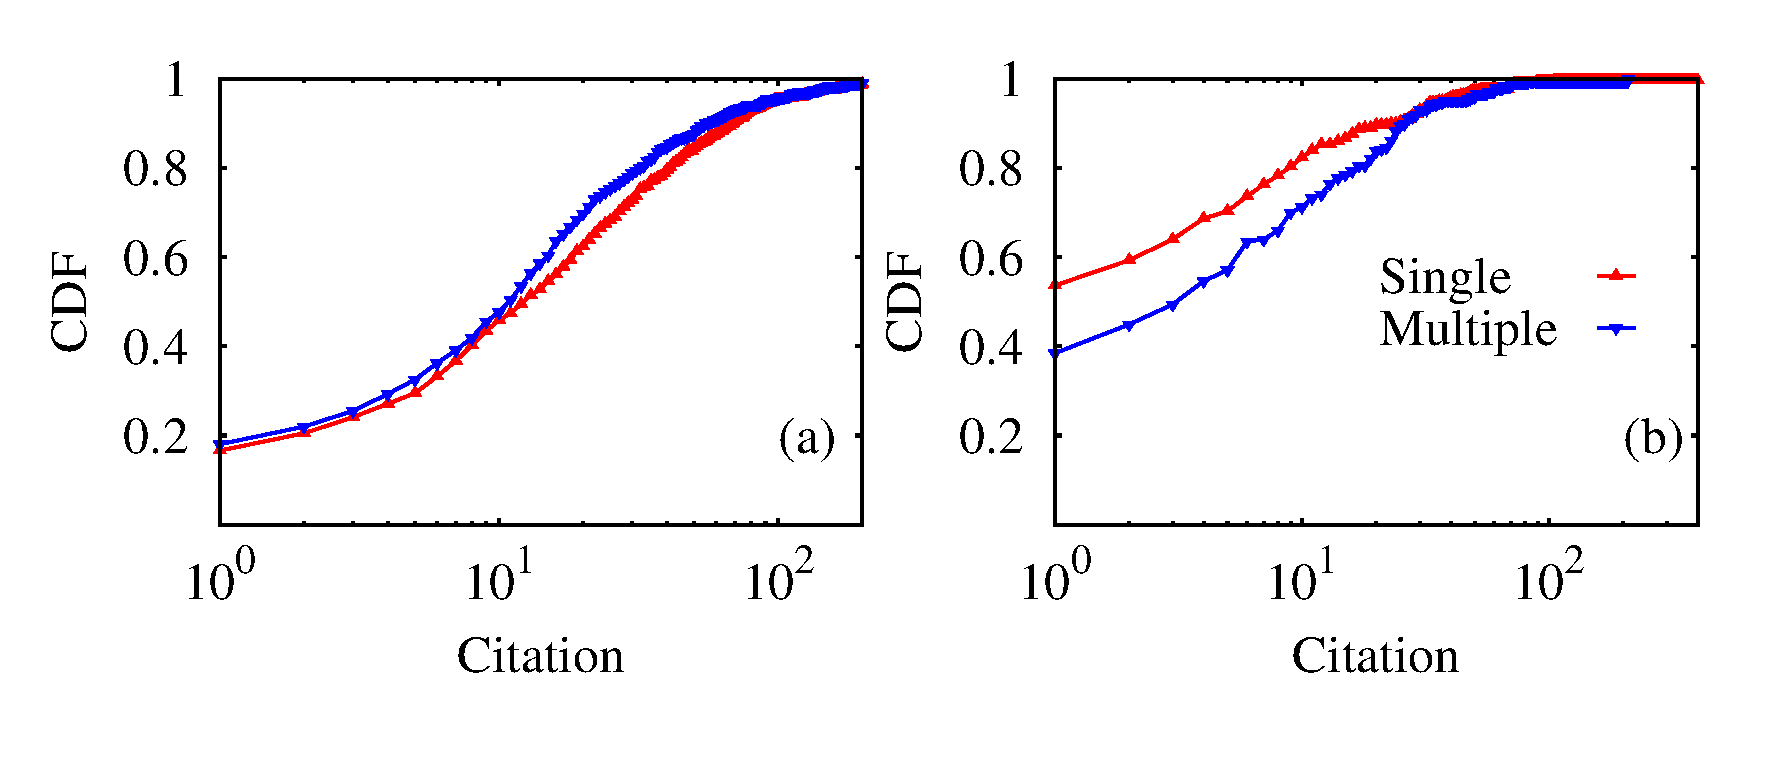
\includegraphics[scale = 0.26]{figures/citation_jhep_1.eps}
 \caption{\label{citation:jhep} Citation distribution of the multi-refereed and single-refereed papers for (Left) accepted and (Right) rejected papers for JHEP dataset.\vspace{-4mm}} 
\end{figure}

\begin{figure}
 \centering
 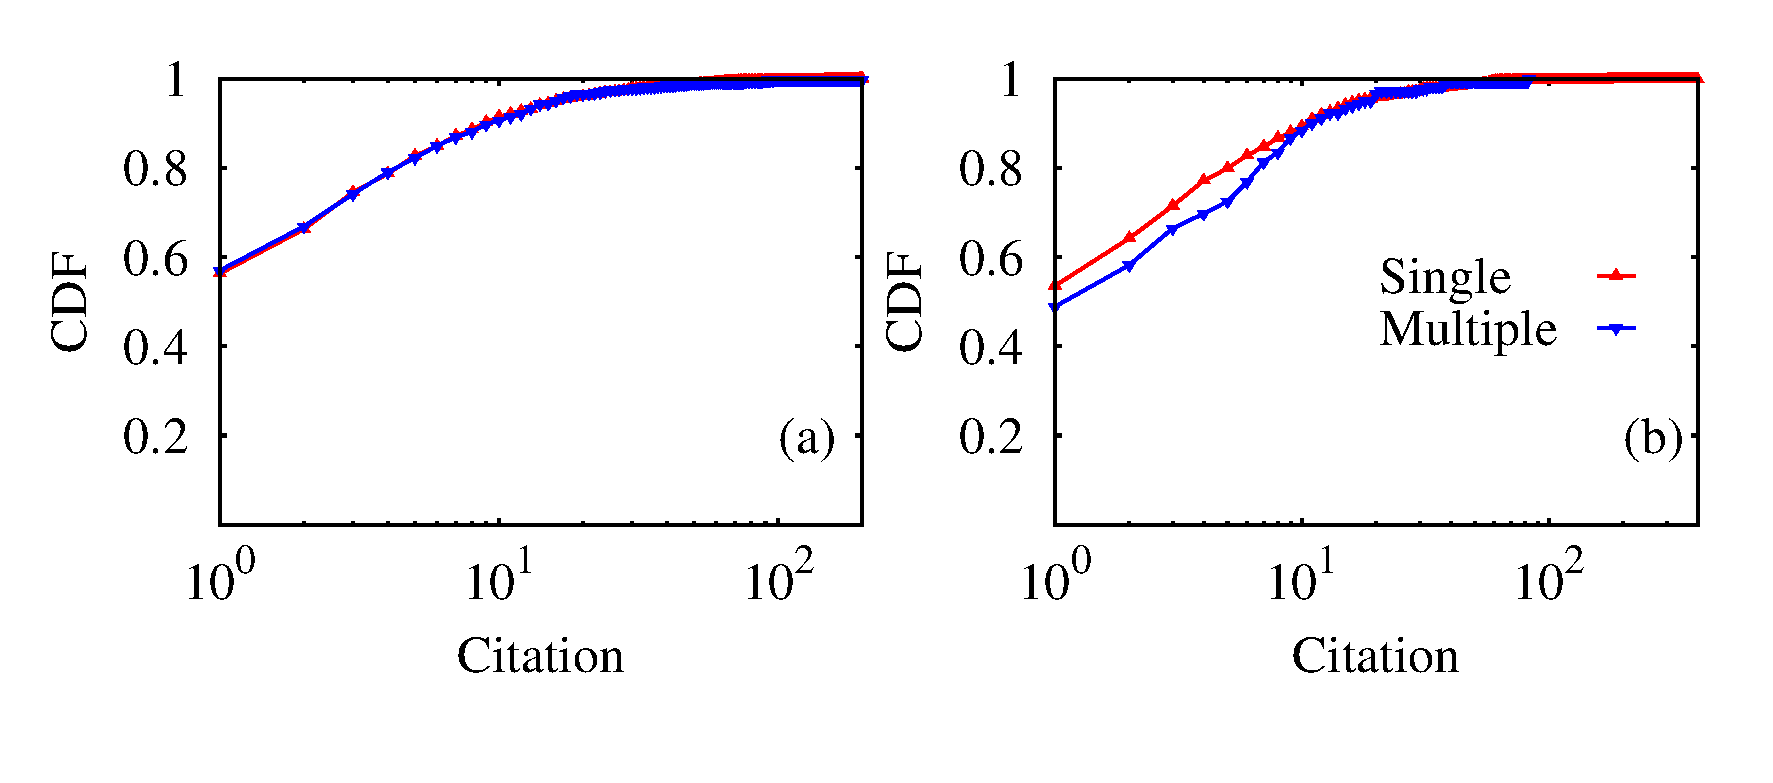
\includegraphics[scale = 0.26]{figures/citation_jstat_1.eps}
 \caption{\label{citation:jstat} Citation distribution of the multi-refereed and single-refereed papers for (Left) accepted and (Right) rejected papers for JSTAT dataset.\vspace{-2mm}}
\end{figure}

\begin{figure}
 \centering
 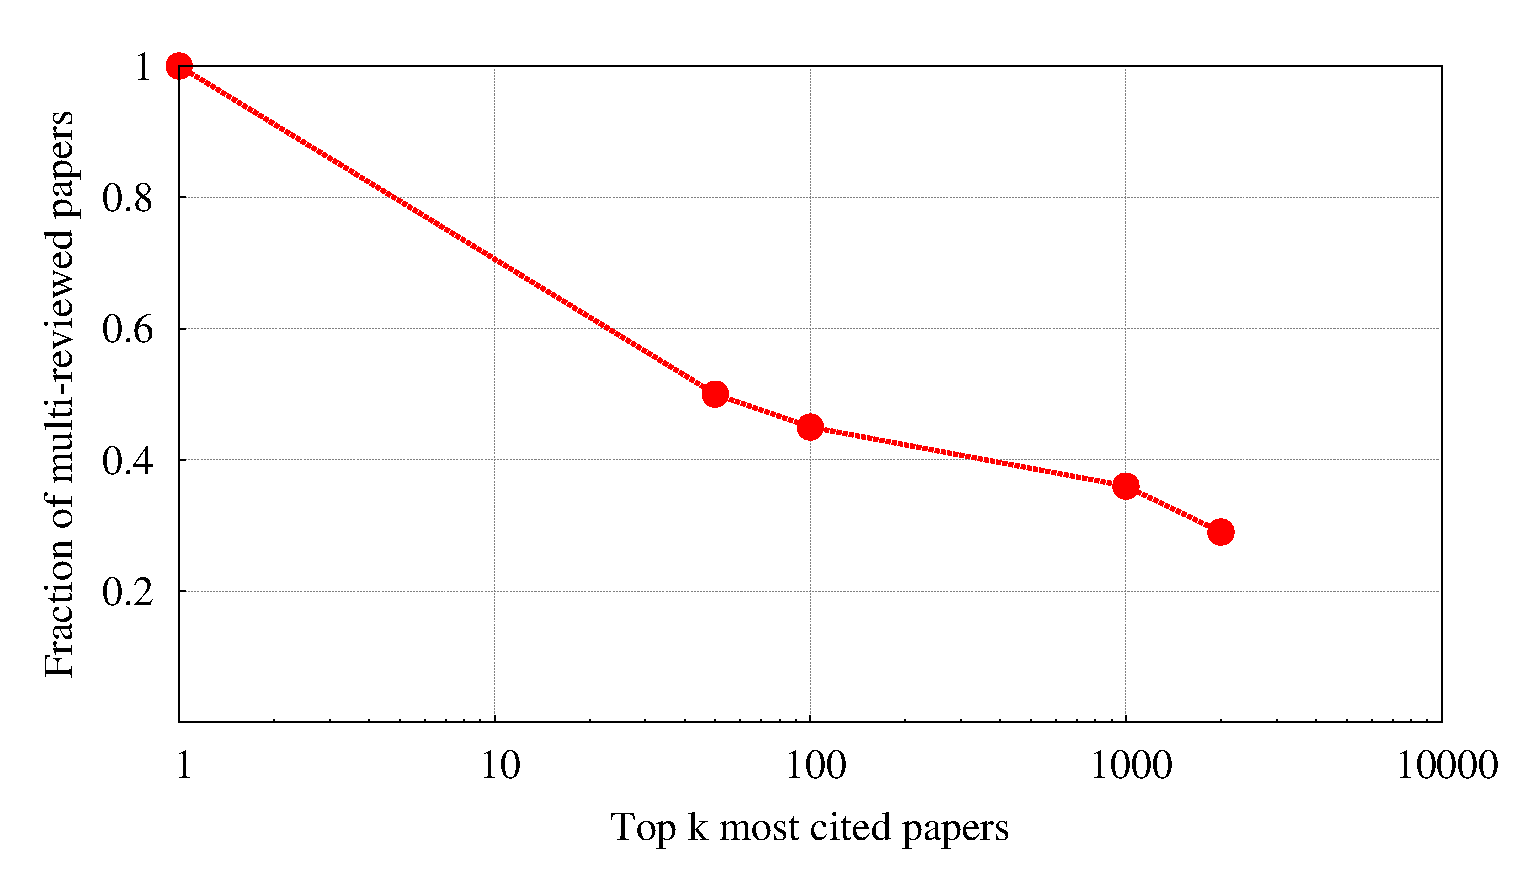
\includegraphics[scale = 0.26]{figures/best_paper.eps}
 \caption{\label{fig:best} Fraction of multi-refereed papers in the top $k$ most cited papers where $k = 1,50,100,500,1000,2000$.\vspace{-4mm}}
\end{figure}

\begin{figure*}[!ht]
 \centering
 \begin{subfigure}[b]{0.49\textwidth}
 \centering
  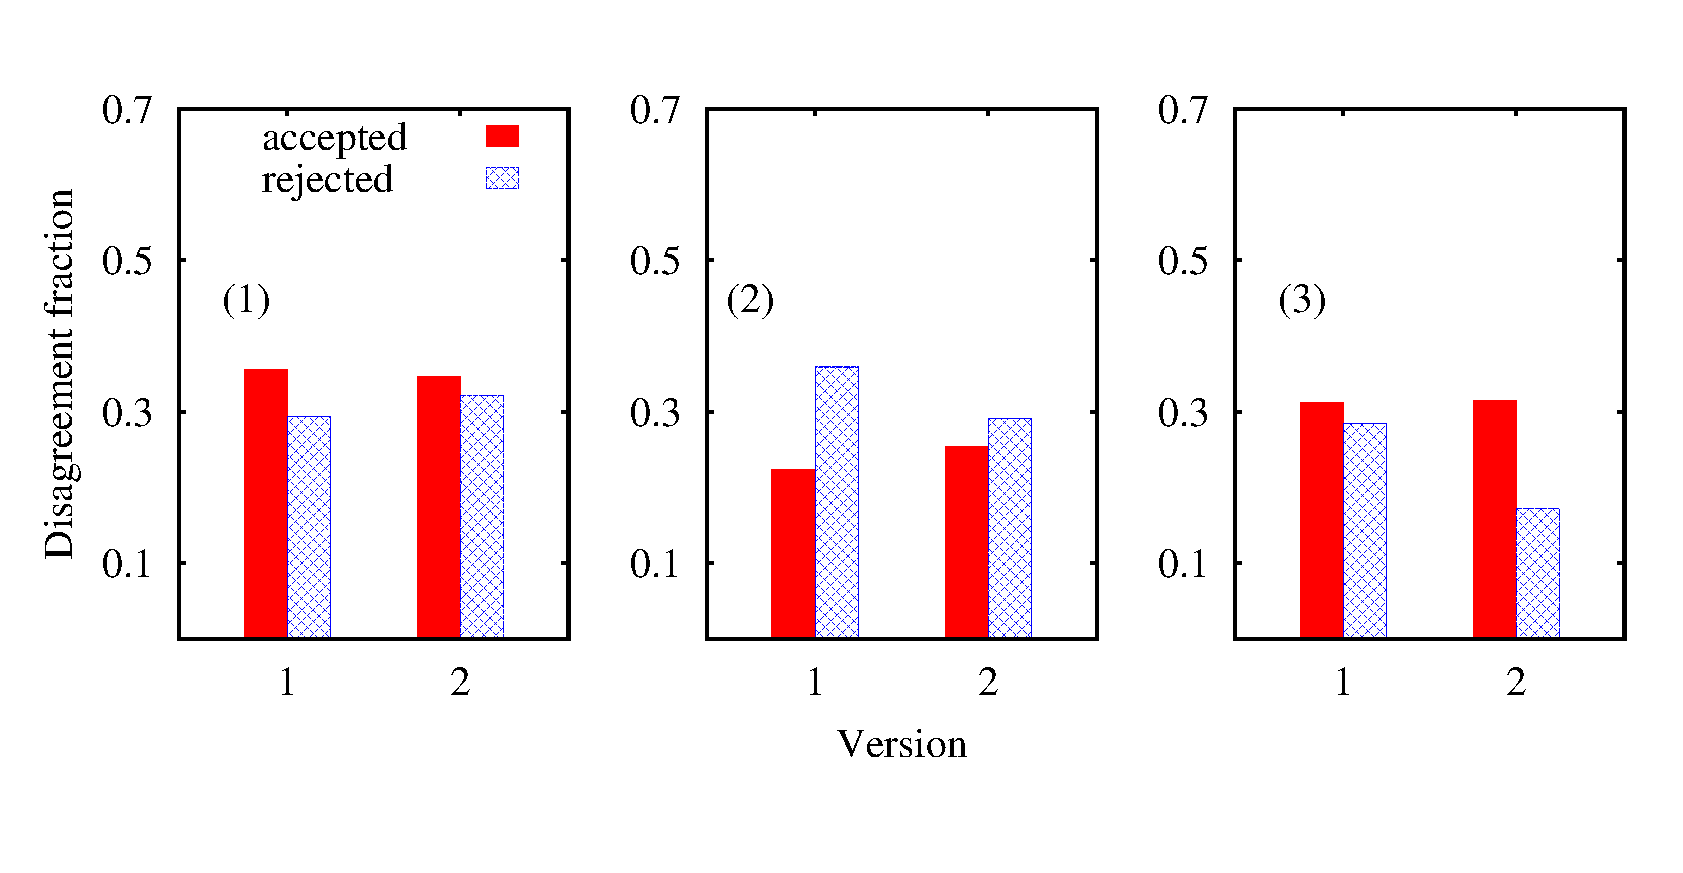
\includegraphics[scale = 0.28]{figures/jhep_all.eps}
  \caption{\label{disagree:jhep}JHEP}
 \end{subfigure}%
 ~
 \begin{subfigure}[b]{0.49\textwidth}
 \centering
  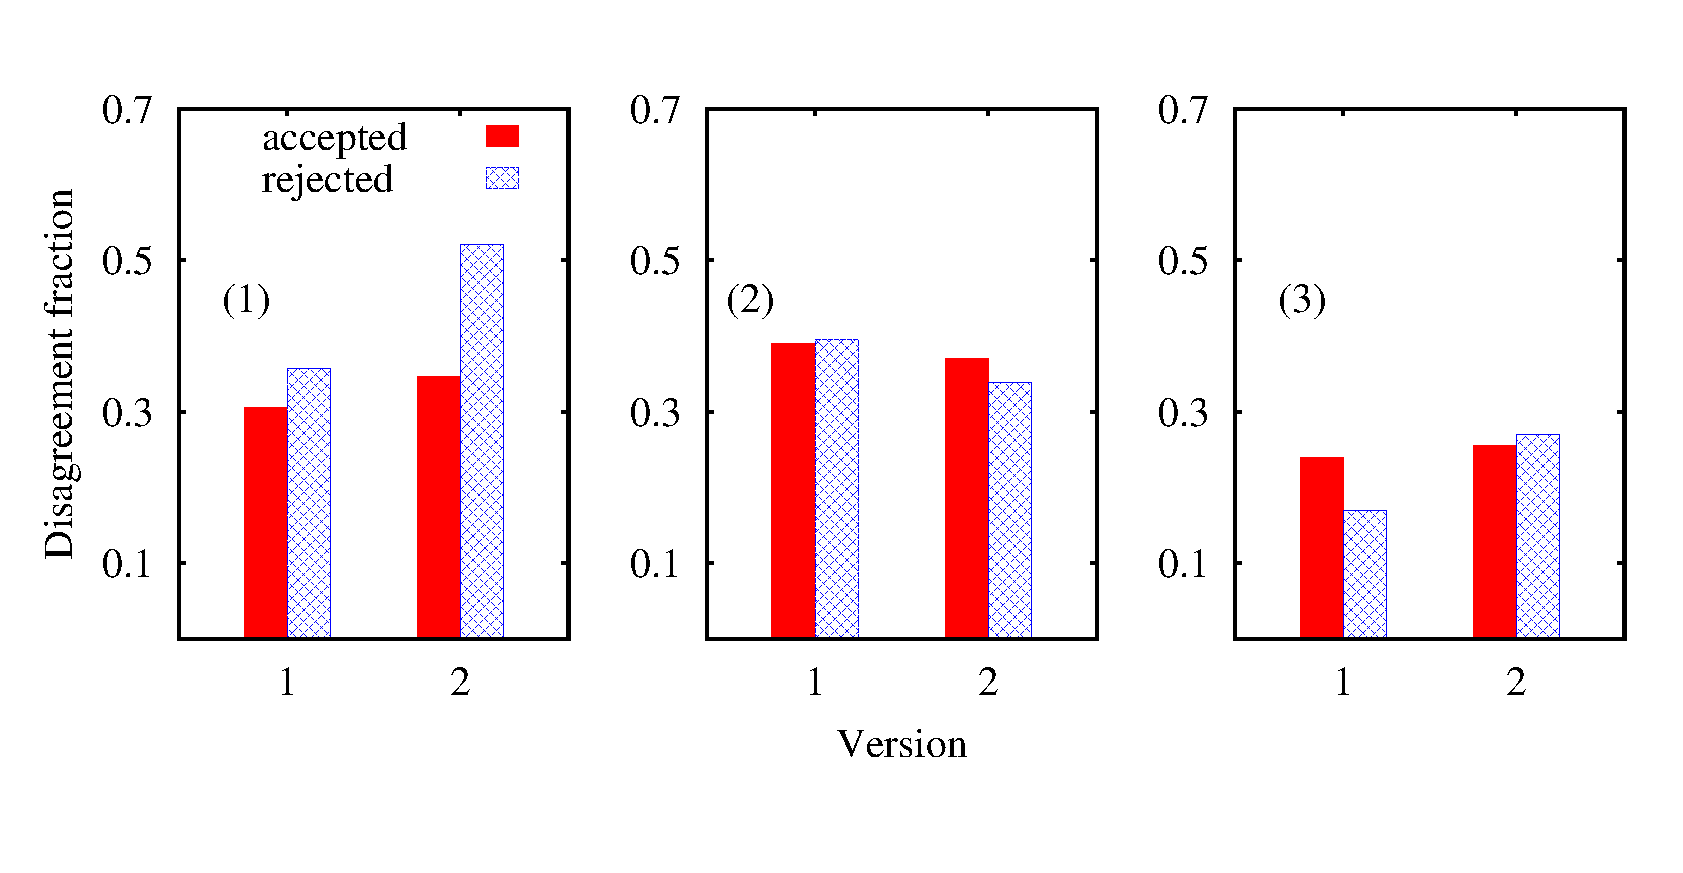
\includegraphics[scale = 0.28]{figures/jstat_all.eps}
  \caption{\label{disagree:jstat}JSTAT}
 \end{subfigure}

 \caption{ Fraction of cases where the reviewers disagreed with respect to (1) length (2) sentiment and (3) content for (a) JHEP and (b) JSTAT 
  datasets.\vspace{-4mm}}
  
\end{figure*}


\medskip
